\documentclass{ctexart}

\usepackage{graphicx}
\usepackage{amsmath}
\usepackage{float}

\title{Programming 2}

\author{洪晨瀚 \\ 信息与计算科学 3200300133}

\begin{document}

\maketitle
\graphicspath{{image/}}



\section*{Interpolation Polynomial Function}
\subsection*{Newton Polynomial}
\begin{verbatim}
  void NewtonMethod(vector<double> a,vector<double> b)
  {
    int n=size(a);
    vector<Comparable> xn;
    vector<Comparable> fn;
    vector<Comparable> A;
    for(int i=0;i<n;i++)
    {
      xn.push_back(a[i]);
      fn.push_back(b[i]);
    }

    A.push_back(fn[0]);
    int m=0;
    int temp=n;
    while(temp!=0)
    {     
      m=m+temp;
      temp=temp-1;
    }

    int l=0;
    temp=2;
    if(n==1)
    {
      A.push_back(fn[0]);
    }
    else 
    {
      while(temp!=n)
      {
	l=l+1;
	temp=temp+1;
      }

      int h=0;
      int k=n-1;
      int count=0;
      for(int i=n;i<m;i++)
      {
	double tempf;
	if(count!=k)
	{
	  tempf=(fn[i-l-1]-fn[i-l-2])/(xn[count+h+1]-xn[count]);
	  fn.push_back(tempf);
	  if(count==0)
	  {
	    A.push_back(tempf);
	  }
	  count=count+1;
	}
	else
	{
	  count=0;
	  k=k-1;
	  l=l-1;
	  h=h+1;
	  tempf=(fn[i-l-1]-fn[i-l-2])/(xn[count+h+1]-xn[count]);
	  fn.push_back(tempf);
	  if(count==0)
	  {
	    A.push_back(tempf);
	  }
	  count=count+1;
	}   	    
      }
    
      int n_p=size(A);
      Comparable p;
      cout<<A[0];
      for(int i=1;i<n_p;i++)  
      {
        cout<<showpos<<A[i];
	for(int j=0;j<i;j++)
	{
	  cout<<"(x"<<showpos<<-xn[j]<<")";
	}
      }
      cout<<endl;
    }
  }
\end{verbatim}

\clearpage
\subsection*{Hermite Polynomial}
\begin{verbatim}
  void Hermite(vector<double> x, vector<double> y, vector<double> z)
  {
    f.resize(x.size()+1);
    for(int i=0;i<=x.size();i++)
    {
      f[i].resize(x.size()+1);
    }
    
    for(int i=0;i<x.size();i++)
    {
      f[i][0]=y[i];
    }

    for(int i=0;i<x.size();i++)
    {
      ans.push_back(x[i]);
    }
    
    for (int i=1;i<x.size();i=i+2)
    {
      f[i][1]=z[i];
    }
    
    for (int i=2;i<x.size();i=i+2)
    {
      f[i][1]=(f[i][0]-f[i-1][0])/(x[i]-x[i-2]);
    }
    
    for (int i=2;i<x.size();i++)
    {
      for (int j=i;j<x.size();j++)
      {
	f[j][i]=(f[j][i-1]-f[j-1][i-1])/(x[j]-x[j-i]);
      }
    }

    cout<<noshowpos<<f[0][0];
    for (int i=1;i<f.size();i++)
    {
      cout<<showpos<<f[i][i];
      for (int j=0;j<i;j++)
      {
	cout<<"(x"<<showpos<<-x[j]<<")";
      }    
    }
    cout<<endl;    
  }
\end{verbatim}

\clearpage
\section*{Question}
\subsection*{B :}
\begin{flushleft}
  Plot $f(x)=\frac{1}{1+x^2}$, for $x\in[-5,5]$, using $x_i=-5+10\frac{i}{n}$, $i=0,1,......,n$, $n=2,4,6,8$ .

  \begin{figure}[H]
  \centering
    \centering
    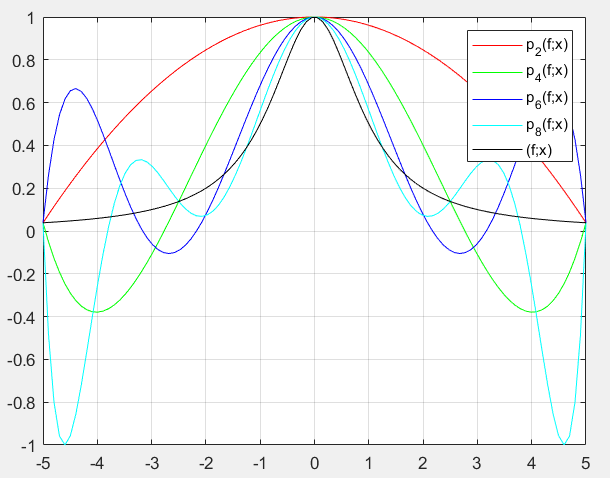
\includegraphics[width=7cm]{1}
    \caption{Runge Phenomenon}
  \end{figure}
\end{flushleft}

\subsection*{C :}
\begin{flushleft}
  Plot $f(x)=\frac{1}{1+25x^2}$, for $x\in[-1,1]$, using $x_k=\cos{\frac{2k-1}{2n}\pi}$, $k=1,2,......,n$, $n=5,10,15,20$ .

  \begin{figure}[H]
  \centering
    \centering
    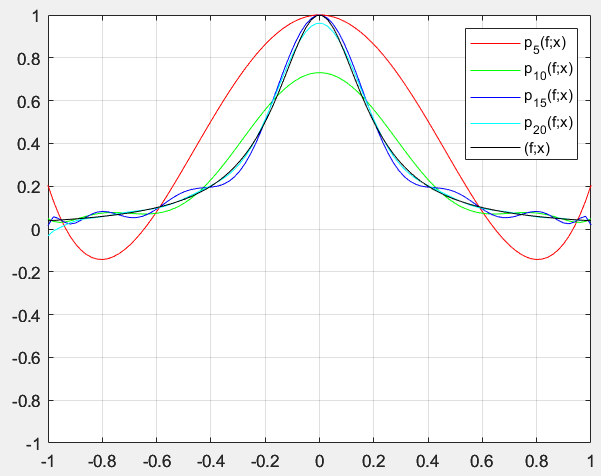
\includegraphics[width=7cm]{2}
    \caption{Chebyshev Interpolation}
  \end{figure}
\end{flushleft}

\subsection*{D :}
\begin{flushleft}
  (a)From \verb|图3| and \verb|图4|, Position of the car and its speed for t=10s are $742.503$ and $48.248$. \\
  (b)The car ever exceeds the 81 feet per second speed limit when t=12. \\
  \begin{figure}[H]
    \centering
    \begin{minipage}[t]{0.48\textwidth}
      \centering
      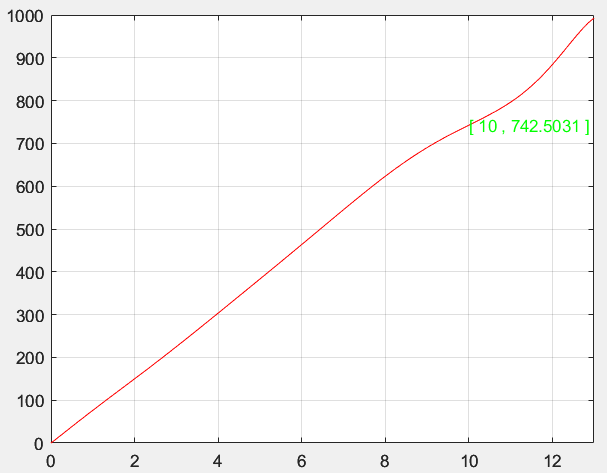
\includegraphics[width=6cm]{3}
      \caption{Position}
    \end{minipage}
    \begin{minipage}[t]{0.48\textwidth}
      \centering
      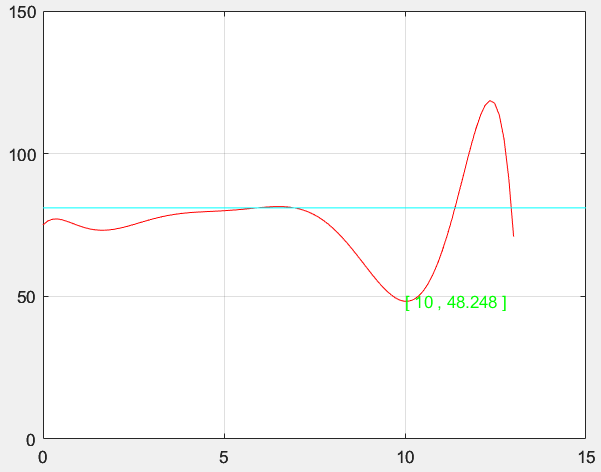
\includegraphics[width=6cm]{4}
      \caption{Speed}
    \end{minipage}
  \end{figure}    
\end{flushleft}

\subsection*{E :}
\begin{flushleft}
  (a) \\
  \begin{figure}[H]
  \centering
    \centering
    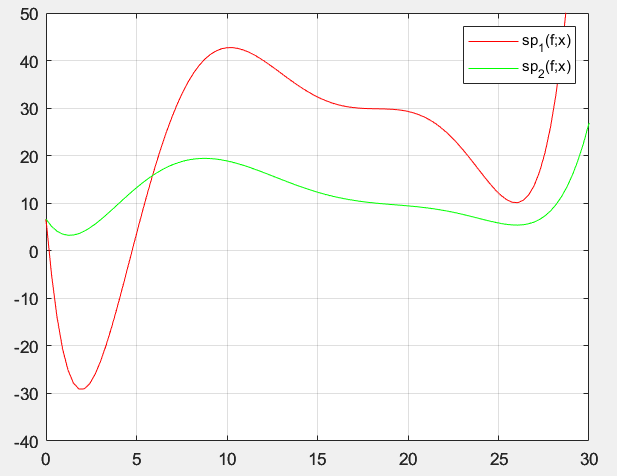
\includegraphics[width=7cm]{5}
    \caption{Runge Phenomenon}
  \end{figure}

  (b)The two samples of larvae will die after another 15 days.
\end{flushleft}

\end{document}
